\documentclass[12pt]{article}
\usepackage[english]{babel}
\usepackage{natbib}
\usepackage{lipsum}
\usepackage{fontawesome}
\usepackage{hyperref}
\usepackage{circuitikz}
\usepackage{url}
\usepackage{placeins}
\usepackage[utf8x]{inputenc} 
\usepackage{amsmath}
\usepackage{graphicx}

\graphicspath{{images/}}
\usepackage{parskip}
\usepackage{fancyhdr}
\usepackage{vmargin}
\usepackage{wrapfig}
\usepackage{subfig}

\usepackage{siunitx}



\setmarginsrb{3 cm}{2.5 cm}{3 cm}{2.5 cm}{1 cm}{1.5 cm}{1 cm}{1.5 cm}


%%%%%%%% to embed code %%%%%%%%%%%%%%
\usepackage{listings}
\usepackage{color}
\definecolor{dkgreen}{rgb}{0,0.6,0}
\definecolor{gray}{rgb}{0.5,0.5,0.5}
\definecolor{mauve}{rgb}{0.58,0,0.82}
\lstset{
  language=Java,
  aboveskip=3mm,
  belowskip=3mm,
  showstringspaces=false,
  columns=flexible,
  basicstyle={\small\ttfamily},
  numberstyle=\tiny\color{gray},
  keywordstyle=\color{blue},
  commentstyle=\color{dkgreen},
  stringstyle=\color{mauve},
  breaklines=true,
  breakatwhitespace=true,
  tabsize=3,
  numbers=left,
  xleftmargin=2em,
  frame=single,
  framexleftmargin=1.5em
}

%%%%%%%% to embed code %%%%%%%%%%%%%%


\title{Portable Heart Rate Monitor}	% Title  
\author{EN1093 - Laboratory Practice}	%Author
\date{\today}						% Date

\makeatletter
\let\thetitle\@title
\let\theauthor\@author
\let\thedate\@date
\makeatother

\pagestyle{fancy}
\fancyhf{}
\rhead{\theauthor}
\lhead{\thetitle}
\cfoot{\thepage}

\begin{document}

%%%%%%%%%%%%%%%%%%%%%%%%%%%%%%%%%%%%%%%%%%%%%%%%%%%%%%%%%%%%%%%%%%%%%%%%%%%%%%%%%%%%%%%%

\begin{titlepage}
	
	\centering
	
	\textsc{\small DEPARTMENT OF ELECTRONIC AND TELECOMMUNICATION ENGINEERING\\}
	\textsc{\small UNIVERSITY OF MORATUWA}\\[1.0 cm]
    \vspace*{0.5 cm}
    
\includegraphics[scale = 0.35]{uom.png}\\[1.5 cm]	% University Logo
    \textsc{\LARGE Group Project Report}\\[0.7 cm]	% University Name 
	\textsc{\Large EN1093 - Laboratory Practice}\\[0.5 cm]			% Course Code

	\rule{\linewidth}{0.2 mm} \\[0.4 cm]
	{ \huge \bfseries \thetitle}\\
	\rule{\linewidth}{0.2 mm} \\[1.5 cm]
	
	\begin{minipage}{0.4\textwidth}
		\begin{flushleft} \large
			\emph{Authors:}\\
			K.K. Herath\\
			H.M.U.D Herath\\
			R.U. Hettiarachchi\\
			M.N. Hettiaratchchi
			\end{flushleft}
			\end{minipage}~
			\begin{minipage}{0.4\textwidth}
			\begin{flushright} \large
			\emph{Registration Number:} \\
			170213V\\
			170215U\\
			170221T\\
			170222X
		\end{flushright}
	\end{minipage}\\[2 cm]
	 This is submitted as a partial fulfillment for the module EN1093\\[0.2 cm]
	 ---\\
	{\large \thedate}\\[2 cm]
	
	\vfill
	
\end{titlepage}

\newpage
\section{Abstract}
The proposed project measures the heart rate of a person using optical sensors. 
The optical sensor detects the variation of blood volume at the fingertip.
In our project the sensor will be an infrared light emitting diode (IR LED) which will be on the same side of the finger.
The underlying principle is that the intensity of the reflected infrared light varies on the blood volume at an instance of the fingertip, which changes proportionately to each cardiac cycle. 
The lighting condition in the environment is very important to avoid distortion in the signal so we have taken the following measures,

• To design a special enclosure to cover the optical sensor for accurate measurements

• To use a band filter to remove unnecessary wavelengths.

Based on the refined output signal, we used an Atmel microcontroller to calculate and display the heart rate through the LCD Display.

\section{Acknowledgement}
We would like to express our gratitude to our supervisor Mr.Asanka Rathnayake for giving us technical advice and guidance.\\
Our sincere thanks goes to Mr.Thilina Sameera Ambagahawaththa for the inspiration and advice given to us to compile this report in LaTeX.

We pay our gratitude to all the lecturers, instructors and other academic staff who intimately welcomed us to share their knowledge and experiences. We are very grateful to the personnel who are in charge of laboratories for allowing us to use the laboratories when needed and for the support given to solve technical problems.

%%%%%%%%%%%%%%%%%%%%%%%%%%%%%%%%%%%%%%%%%%%%%%%%%%%%%%%%%%%%%%%%%%%%%%%%%%%%%%%%%%%%%%%%%
\newpage
\tableofcontents
\pagebreak
%%%%%%%%%%%%%%%%%%%%%%%%%%%%%%%%%%%%%%%%%%%%%%%%%%%%%%%%%%%%%%%%%%%%%%%%%%%%%%%%%%%%%%%%%


%%%%%%%%%%%%%%%%%%%%%%%%%%%%%%%%%%%%%%%%%%%%%%%%%%%%%%%%%%%%%%%%%%%%%%%%%%%%%%%%%%%%%%%%%
\section{Introduction}
Heart rate is the number of times one’s heart beats per minute.The portable heart rate monitor is a personal monitoring device that measures the heart rate in real time. For an average person this value lies between 60-100 bpm. The heart rate rises gradually during excercises and returns slowly to the rest value after excercise. The rate when the pulse returns to normal is an indication of fitness in a person.  Therefore a heart rate monitor is an essential device nowadays to keep in track with your body not only for someone who is suffering with heart diseases but also for a normal person to maintain fitness. Having a portable heart rate monitor makes it easy to carry it around when travelling. 
\\
In this project reflective photoplethysmogram(PPG) is used for heart rate monitoring. These sensors uses a light based technology to sense the rate of blood flow as controlled by the heart’s pumping action. This method is less sensitive to motion artifacts and therefore is user friendly.
\\

%%%%%%%%%%%%%%%%%%%%%%%%%%%%%%%%%%%%%%%%%%%%%%%%%%%%%%%%%%%%%%%%%%%%%%%%%%%%%%%%%%%%%%%%%








%%%%%%%%%%%%%%%%%%%%%%%%%%%%%%%%%%%%%%%%%%%%%%%%%%%%%%%%%%%%%%%%%%
\newpage
\section{Methodology}

	\begin{figure}[!htbp]  %this figure will be at the right
		\centering
		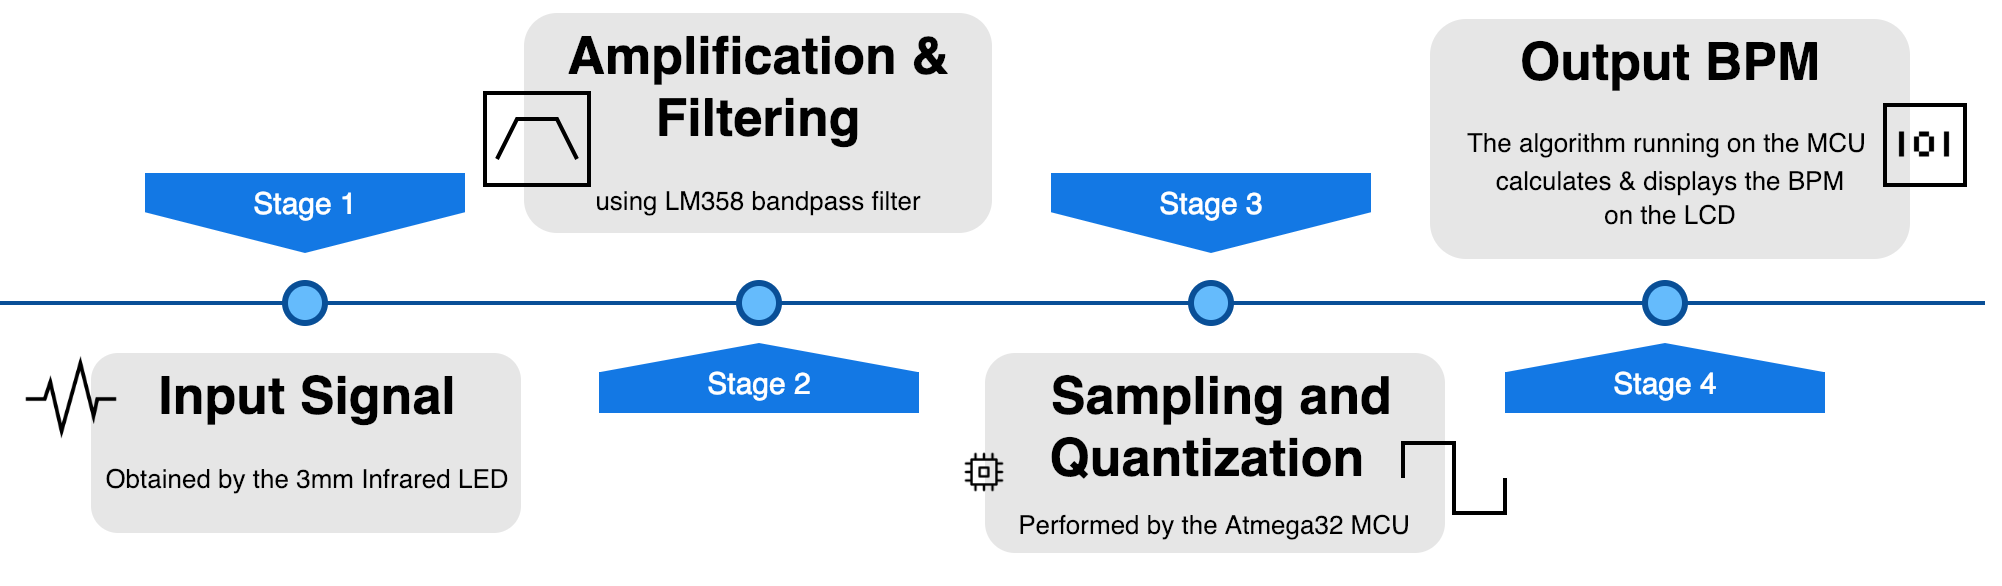
\includegraphics[width=1\textwidth]{block_summary}
		\caption{Methodology in a nutshell}
	\end{figure}

	\subsection{Sensor - (principle)}
	
	\begin{figure}[!htbp]  %this figure will be at the right

		\centering
		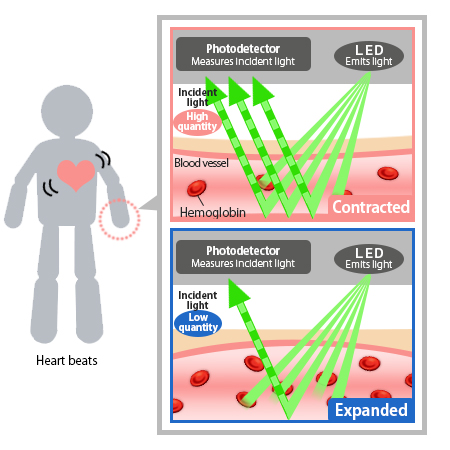
\includegraphics[width=0.65\textwidth]{sensing.jpg}
		\caption{How IR LED light is reflected from the blood vessels\cite{epson_sensor}}
	\end{figure}


		\subsection{Amplification and Filtering}
		
		To amplify the PPG signal we designed an amplifier circuit. However we observed that without proper filtering we cannot get a clear signal due to noise.
		So we had to determine the necessary values for the filter circuit.\\
		The typical heart rate of an adult is between 60-100bpm\cite{typical_pulse}.In frequency terms, these values correspond to the range 1-1.7 Hz.So an active bandpass filter circuit was designed to provide the following characteristics using LM358.


\subsubsection{Calculations}
\label{sec:4.2.1}
\begin{center}
	Cutoff frequency ($f$) = $\frac{1}{2\pi RC}$
	
	
	
	Upper cutoff frequency =$\ \frac{1}{2\pi ( 680\ k\si{\ohm}\ )( 100\ nF)}$ = 2.34051 Hz
	
	
	
	Lower cutoff frequency =$\ \frac{1}{2 \pi  ( 47\ k\si{\ohm})( 4.7\ \si{\micro}F)}$ = 0.720484 Hz
	\end{center}
	
	
	
	
	
	So we have a,

		\begin{itemize}
			\item Gain of 10
			\item Lower Cutoff Frequency of 0.72 Hz
			\item Upper Cutoff Frequency of 2.34 Hz\\
		  \end{itemize}
		 To have a low powered operational amplifier we selected LM358 integrated circuit.
	
		\begin{figure}[!htbp]
			\includegraphics[width=\textwidth]{LM358-Bandpass}
			\caption{Active bandpass filter for the pulse sensor}
		\end{figure}
	
		\clearpage
	\subsection{Calculating BPM from the analog signal}
	The ATMega32 microcontroller was used to sample the analog signal to 0-1023 voltage levels. Then an algorithm was developed to identify peaks and thereby calculate the beats per minute. We used Atmel Studio to compile and flash the hex file to the microcontroller. 


	\subsubsection{Microcontroller}
	The ATmega32 is a low power high performance atmel AVR 8-bit microcontroller.
			\begin{figure}[!htbp]
				\centering
				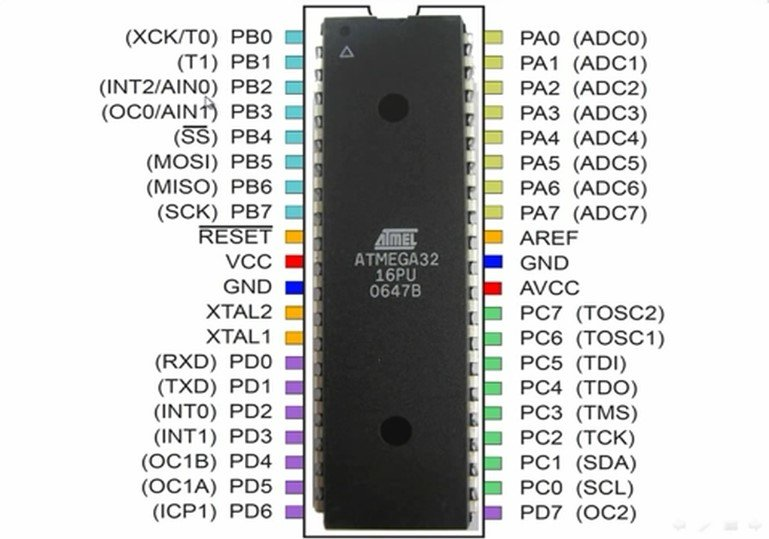
\includegraphics[scale = 1]{atmega32.jpg}
				\caption{ATmega32 pinout}
			\end{figure}
	
		
	\subsubsection{Obtaining a threshold value}
	\label{sec:4.3.2}
			
	\begin{center}
	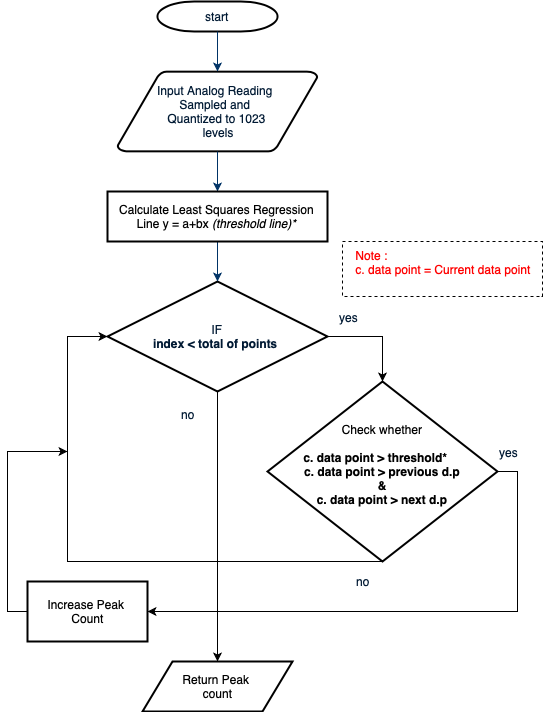
\includegraphics[scale=0.9]{peak_count}
	\end{center}

	The above flowchart explains the peak counting algorithm with automatic threshold calculation. For calculating the threshold we're calculating the least squares regression line.
		

	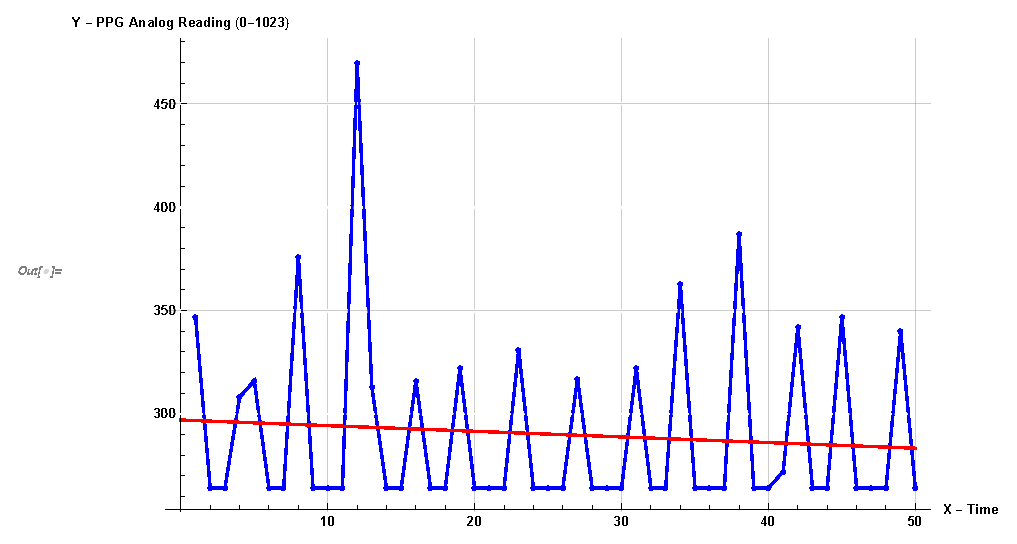
\includegraphics[scale=0.8]{simulation1_gr1.eps}\\
	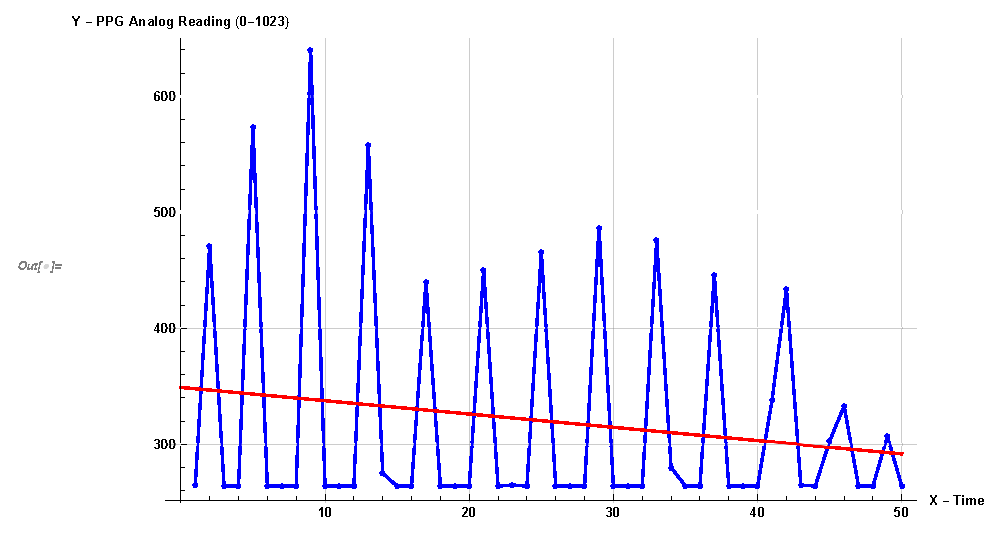
\includegraphics[scale=0.81]{simulation1_gr2.eps}
	\captionof{figure}{Determining threshold value line using simple linear regression}

	In the above graphs, we've presented two data sets of two people and how the threshold line(Red) was obtained.

	\subsubsection{C Code}

	\begin{lstlisting}
		/*  Group 7 | UoM | ENTC 17Batch  
		Complete Code - with debugging notes */
		#ifndef F_CPU
		#define F_CPU 16000000UL // 16 MHz clock speed
		#endif
		
		#define D0 eS_PORTD0
		#define D1 eS_PORTD1
		#define D2 eS_PORTD2
		#define D3 eS_PORTD3
		#define D4 eS_PORTD4
		#define D5 eS_PORTD5
		#define D6 eS_PORTD6
		#define D7 eS_PORTD7
		#define RS eS_PORTC6
		#define EN eS_PORTC7
		
		#include <avr/io.h>
		#include <util/delay.h>
		#include "stdlib.h"
		#include "string.h"
		#include "lcd.h"
		
		char disp[16]="0000000000000001";
		char result[8] = "00000001"; 
		
		
		void lcd_disp(char data_points[],int r,int c,char w[]){ 
		
			if(w=="clear")Lcd8_Clear();
			Lcd8_Set_Cursor(r,c);
			Lcd8_Write_String(data_points);
		}
		
		void ADC_Init(){
			DDRA=0x0;			/* Make ADC port as input */
			ADCSRA = 0x87;			/* Enable ADC, fr/128  */
			ADMUX = 0x40;			/* Vref: Avcc, ADC channel: 0 */
		}
		
		int ADC_Read(char channel){
			int Ain,AinLow;
			
			ADMUX=ADMUX|(channel & 0x0f);	/* Set input channel to read */
		
			ADCSRA |= (1<<ADSC);		/* Start conversion */
			while((ADCSRA&(1<<ADIF))==0);	/* Monitor end of conversion interrupt */
			_delay_us(10);
			AinLow = (int)ADCL;		/* Read lower byte*/
			Ain = (int)ADCH*256;		/* Read higher 2 bits and 
							Multiply with weight */
			Ain = Ain + AinLow;				
			return(Ain);			/* Return digital value*/
		}
		
		/*************** threshold ***************/
		double m=0,c=0; // gradient and slope
		
		double sumit(int data_points[],int length){
			 int i;
			 double sum=0;
			 for(int i=1;i<=length;i++)sum+=data_points[i];
		
			 return sum;
		}
		
		double xysum(int data_points[],int length){
			 int i;
			 double sum=0;
			 for(int i=1;i<=length;i++)sum+=(i)*data_points[i];
		
			 return sum;
		}
		
		void regression(int data_points[],double n){
			double squarex= (n)*(n+1)*(2*n+1)/6.0;
			double xbar = (n+1)/2.0;
			double ybar = sumit(data_points,n)/n;
			
			//printf(" xbar=%f, ybar=%f, squarex=%f, xysum =%f\n",xbar,ybar,squarex,xysum(data_points,n));
		
			m=(xysum(data_points,n)- n*xbar*ybar)/( squarex - n*xbar*xbar );
			c=ybar-m*xbar;
		}
		/*************** end threshold ***************/
		
		
		int main(void){
			DDRD = 0xFF;  // #
			DDRC = 0xFF;  //for lcd
			DDRA = 0x00;  //Analog input
			
			
			ADC_Init();
			//ADMUX = 0b01100000; // Configure ADC to be left justified, use AVCC as reference, and select ADC0 as ADC input
			//ADCSRA = 0b10000111; // Enable the ADC and set the prescaler to max value (128)
		
		
			Lcd8_Init(); //Initializing the LCD screen
			lcd_disp("Starting Pulse ~)",1,0,"");
			lcd_disp("Sensor *_*",2,0,"");
		
			_delay_ms(1000);
			
			lcd_disp("Place your",1,0,"clear");
			lcd_disp("fingertip",2,0,"");
			_delay_ms(2000);
			
			lcd_disp("Keep placing ~",1,0,"clear");
			lcd_disp("your fingertip",2,0,"");
			
			_delay_ms(3000);
			int i;
			int thresh=300;
			int count=0;
			int count2=0; //modified peak counting algo
			
			
			/*  timing data */
				double sampling_rate = 0.100 ;	   	// actually this is the _delay_ms val
				int time_limit = 10 ;  				 //in seconds
				int se=time_limit/(sampling_rate*2);
				int data_points[se+1];
		
			data_points[0]=0;
			/* /timing data */
		
		
			
			/* for debugging purposes -> h and l records the peaks */
			int h=0;
			int l=1023;
			
			char val[6]; //temporary variable for itoa
		
			
			for(i=0;i<time_limit/(sampling_rate*2);i++){	
				data_points[i+1]=ADC_Read(0);
				
				itoa(data_points[i+1],val,10);
				//lcd_disp(val,1,0,"");
				lcd_disp("Measuring.. *_*",1,0,"clear");
				
				int k=16*(data_points[i+1]-200)/375;
				
				char anim[16]="";
				
				int h=0;
				for(h=0;h<k;h++){
					anim[h]='~';
				}
				itoa(k,val,10);
				lcd_disp(anim,2,0,"");
				_delay_ms(sampling_rate*1000);
			
			}
			/*
			for(i=0;i<10;i++){
				lcd_disp("*_*,",5,0,"clear");
				_delay_ms(500);
				lcd_disp("0_0,",5,0,"clear");
				_delay_ms(500);
				lcd_disp("*_-,",5,0,"clear");
				_delay_ms(500);
			}
		*/
		
			regression(data_points,se);
		/* 	Debug code below
			lcd_disp("regression",1,0,"clear");
		
		
			char out[16]="";
			itoa(m*1000,val,10);
			strcat(out,"m= ");
			strcat(out,val);
			strcat(out," ; c= ");
			itoa(c*1000,val,10);
			strcat(out,val);
			lcd_disp(out,2,0,"");	
			_delay_ms(5000);
		*/
			//recorded wave form
			for(i=0;i<time_limit/(sampling_rate*2);i++){	
				thresh=(i+2)*m+c;
		
				int a=data_points[i+1];//current value
				char temp[11]="";
				char ccount[3];
		
				if(a>h)h=a; //max peak
				if(a<l)l=a; //min peak
				
				if(a>thresh){
					count+=1; //peak counting]
					if(a>data_points[i] && a>data_points[i+2]){
						count2+=1;
					}
					
				}
				/* debug code
				
					itoa(count,ccount,10);
					itoa(a,val,10);
					
			 
				strcat(temp,val);
				strcat(temp," - ");
				strcat(temp,ccount);
				itoa(count2,ccount,10);
				strcat(temp,",");
				strcat(temp,ccount);
				lcd_disp(temp,1,0,"clear");
				_delay_ms(100); */
			
			}
			//displaying statistics of the waveform
		/*	char peaks[10]="H- ";	 //maximum value
				itoa(h,val,10);
			strcat(peaks,val);
			strcat(peaks,"; L- ");  //minimum value
				itoa(l,val,10);
			strcat(peaks,val);
			lcd_disp(peaks,1,0,"");
			
			*/
		
		
			//displaying the heart rate
			char bpm[10]="Heart Rate : ";
			
			/*itoa(count*(60/time_limit),val,10);
			
			strcat(bpm,val);
			strcat(bpm," ; N-");
		
			*/
			lcd_disp(bpm,1,0,"clear");
			
			itoa(count2*(60/time_limit),val,10);
		
			strcat(val," bpm");
			lcd_disp(val,2,4,"");
		
		
		}
	\end{lstlisting}
		Based on this \cite{avr_analog} and this data-sheet \cite{atmega32_datasheet}
		%% Calibration and Ambient Lighting conditions %% 


\subsection{Enclosure and PCB Design}

	




\newpage
\section{Implementation and Results}


\subsection{The effect of noise on the signal}
Initially our goal was to amplify the signal received from the photodiodes. Then we observed that we could not receive a clear amplified heartbeat signal as it gets suppressed by the 50Hz noise signal.

\subsubsection{Without the filter - Dominant 50Hz noise}

\begin{figure}[!htbp]
	\begin{tabular}{cc}
	\centering

	\subfloat[oscilloscope output]{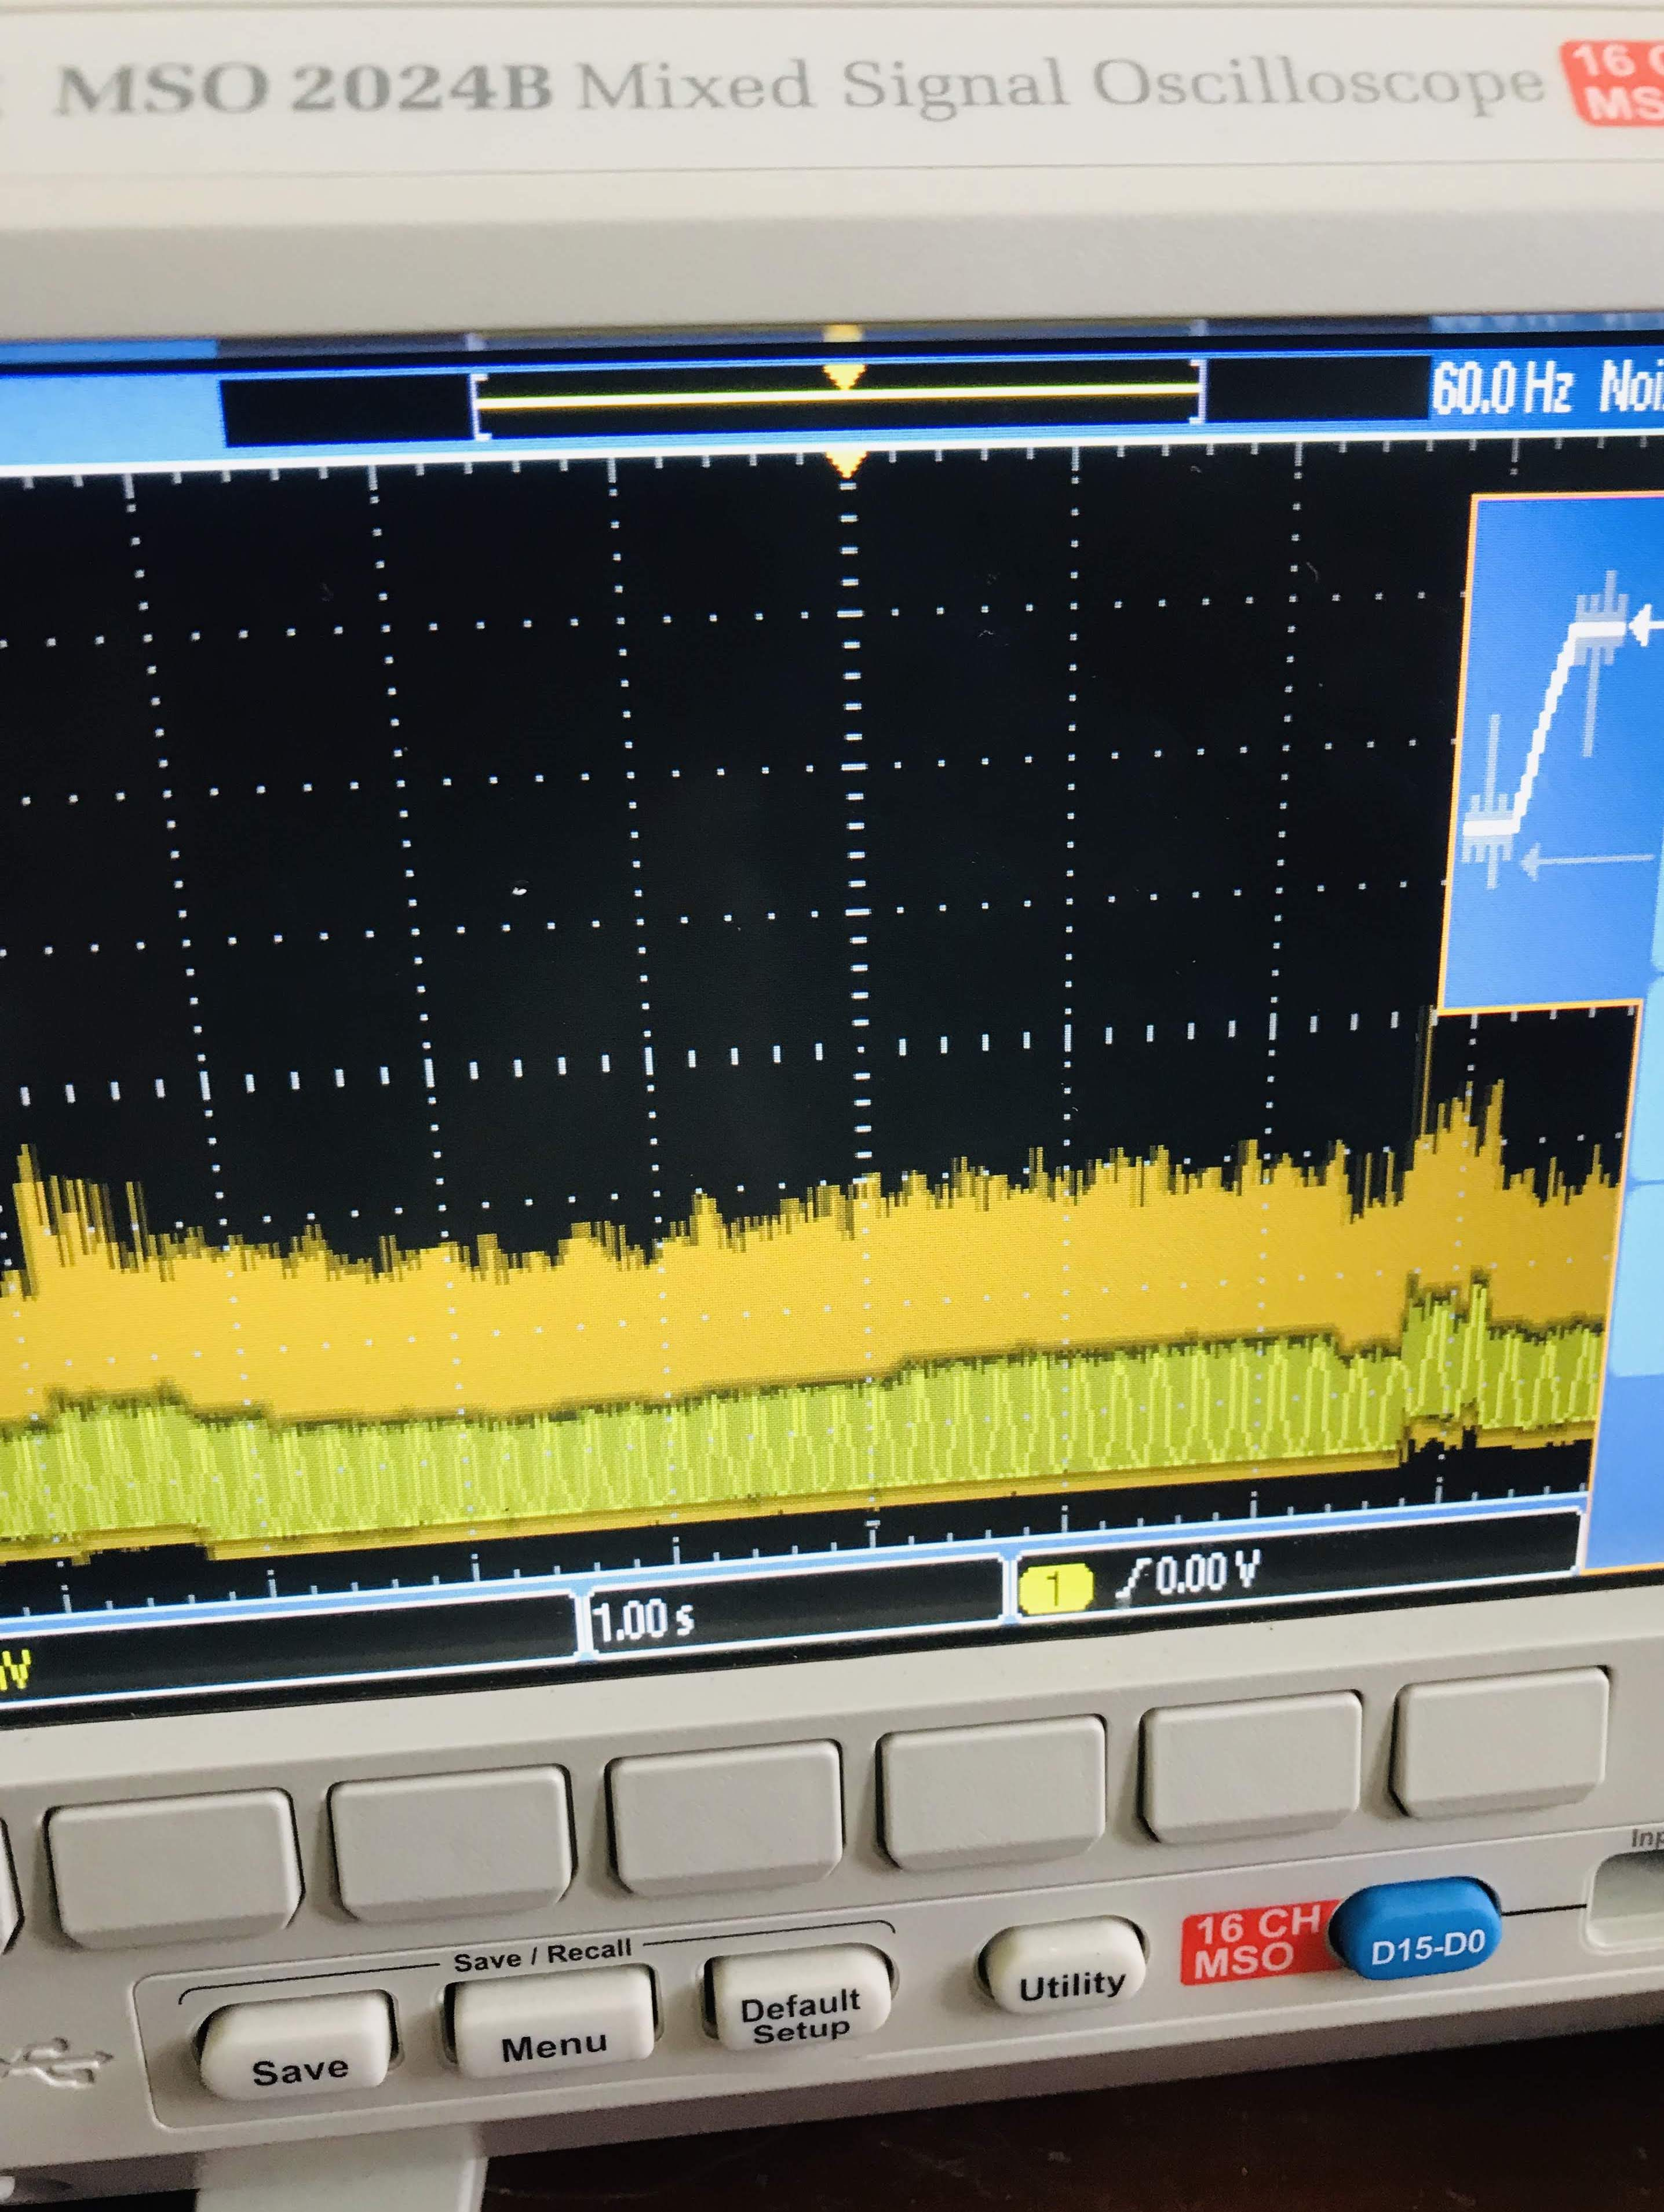
\includegraphics[width = 3in]{50Hz.jpg}}&
\subfloat[zoomed view]{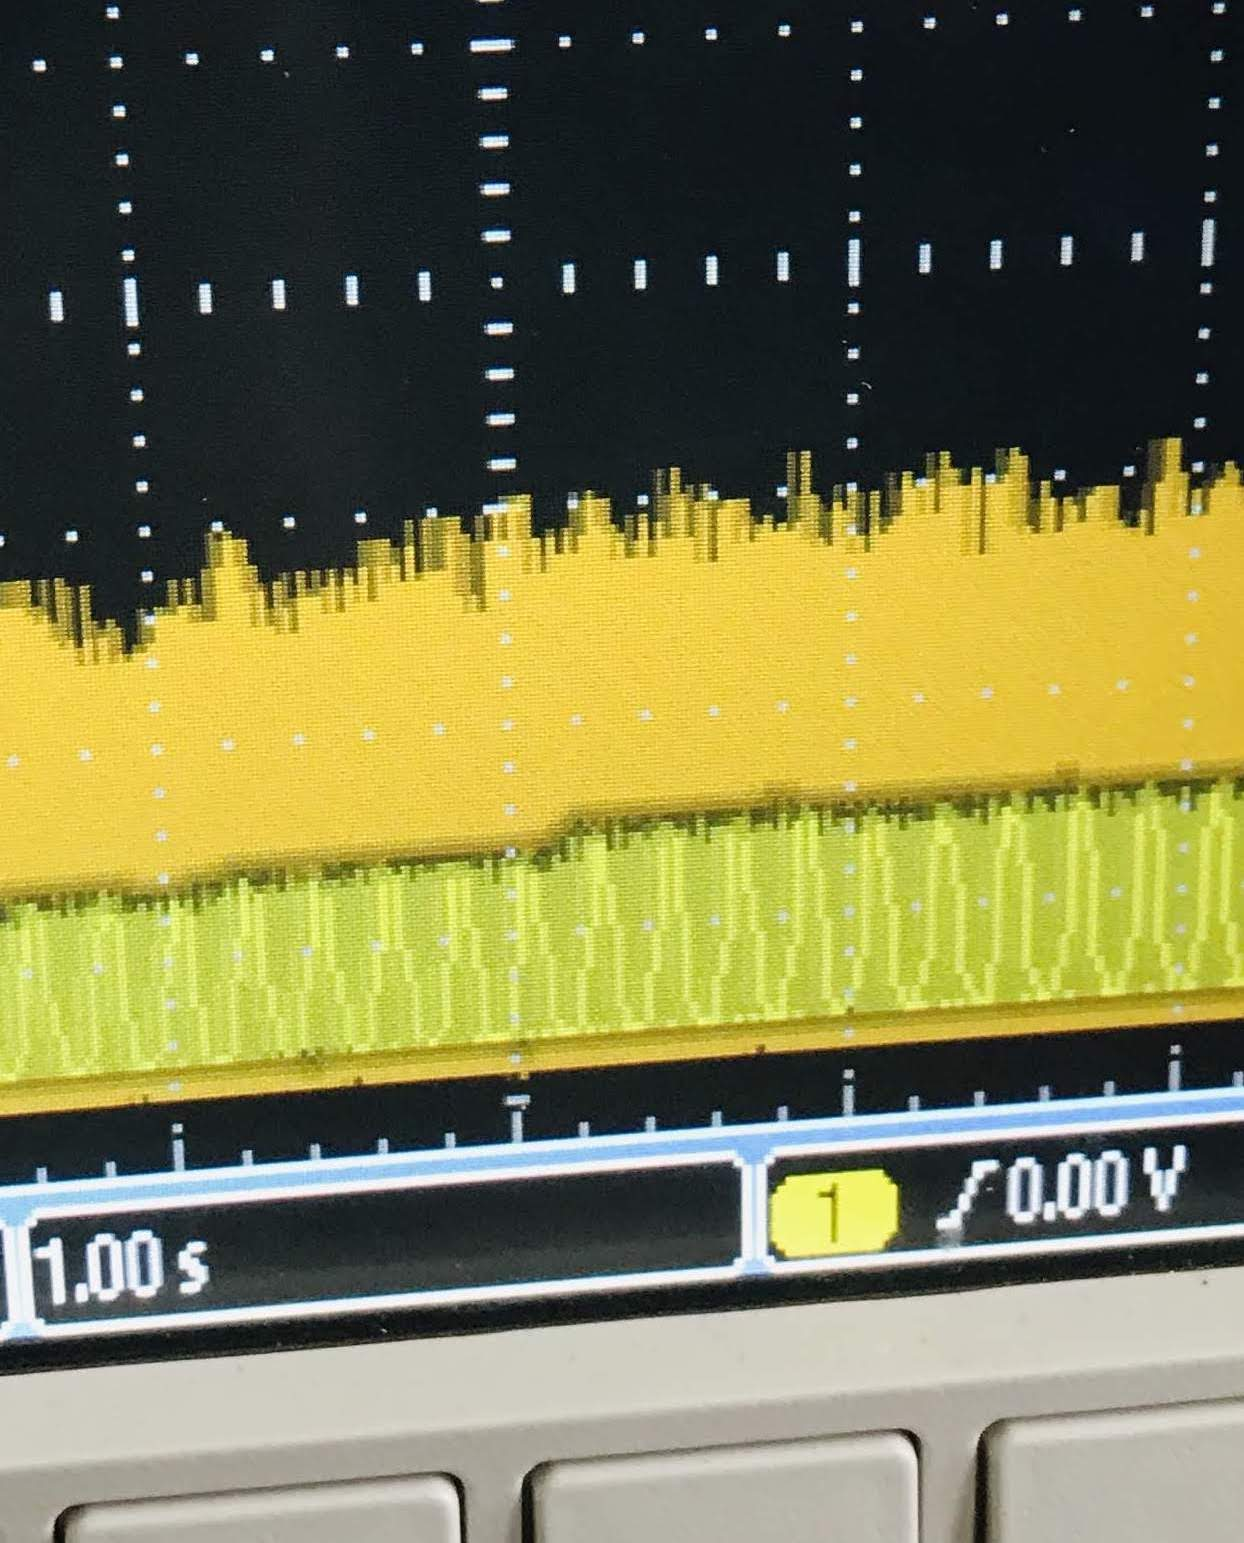
\includegraphics[width = 3in]{50Hz-z.jpg}}\\


	\end{tabular}
\end{figure}

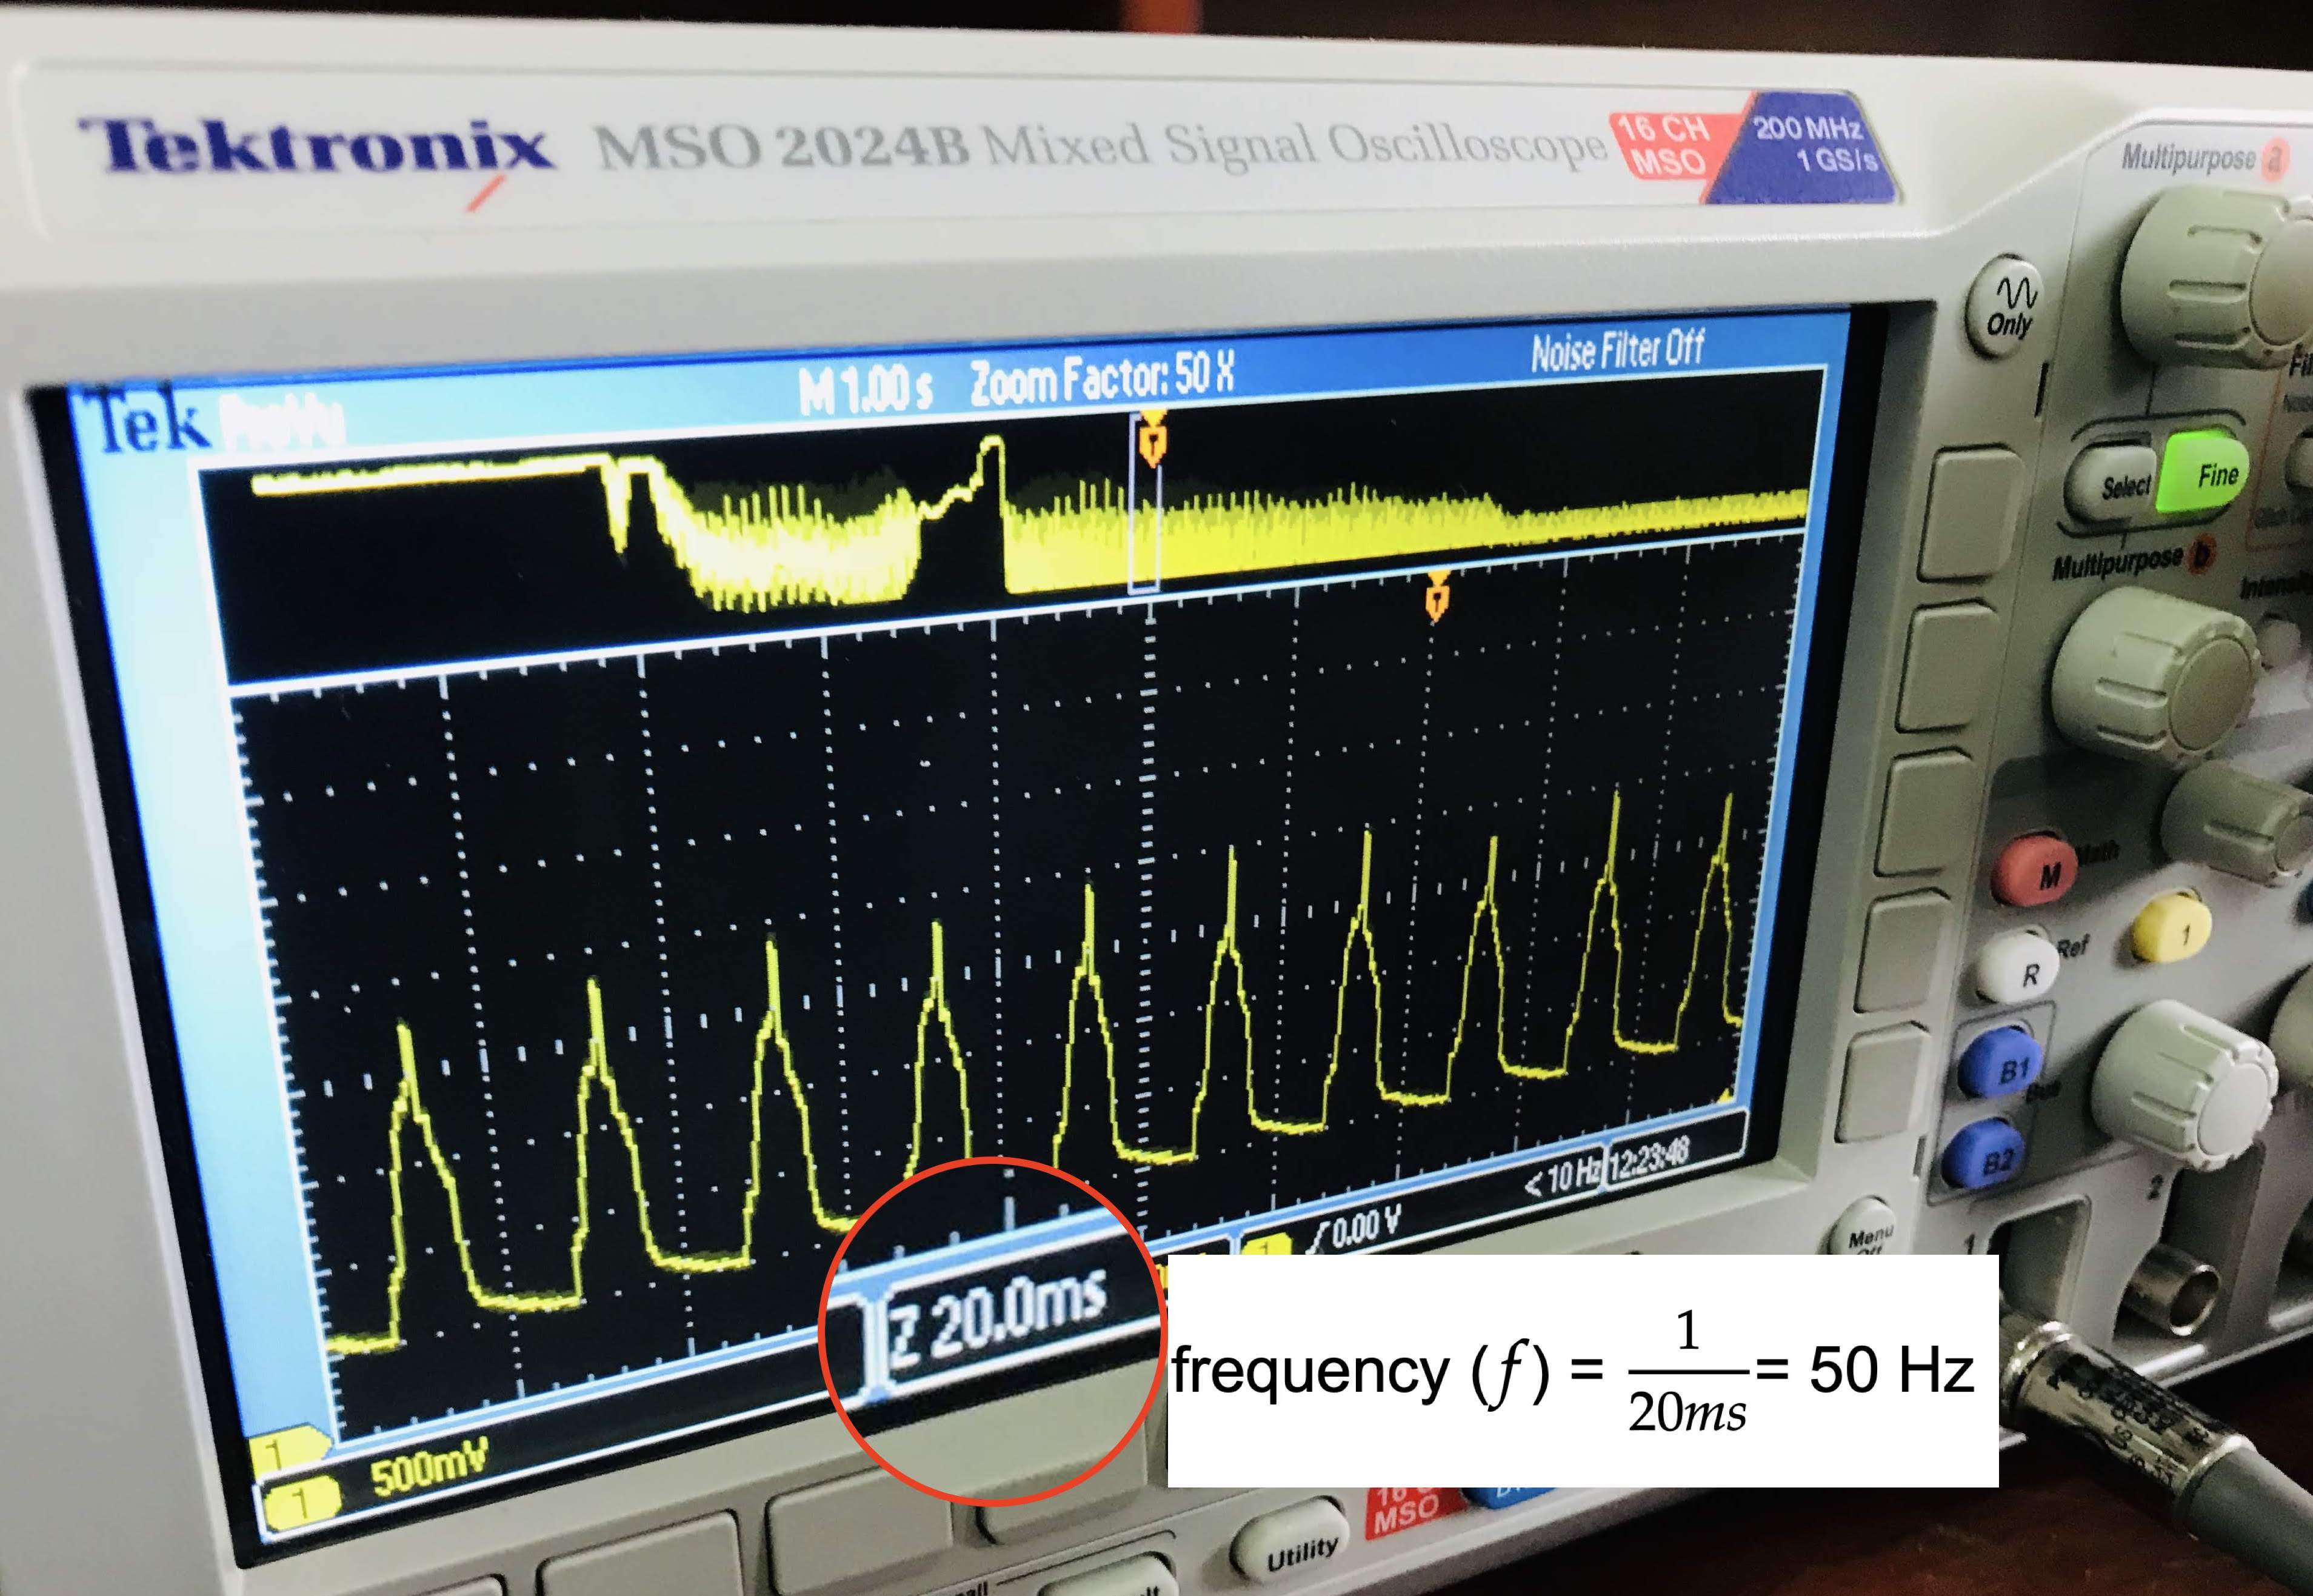
\includegraphics[scale=0.11]{50-dom.jpg}



\subsubsection{With the active bandpass filter}
The initial circuit was modified into an active bandpass filter circuit by calculating the necessary values as shown in \hyperref[sec:4.2.1]{4.2.1}.Next, using the signal generator, the characteristics of our filter circuit from the digital oscilloscope was observed. The responses were as follows;\\ Observation: The amplitudes of the frequencies at the cut off frequencies were gradually reduced.\footnote{The required range of frequencies 50-140bpm (0.83 - 2.33Hz) were passed without much attenuation}

\begin{figure}[h]
 
	\begin{tabular}{ccc}

\subfloat[0.1Hz]{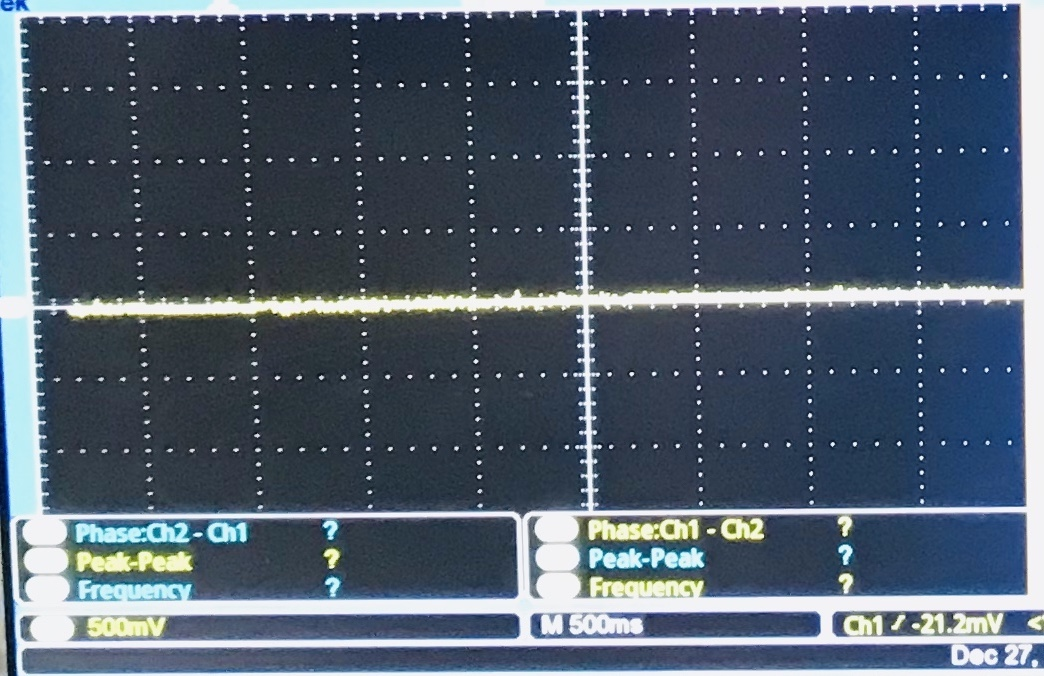
\includegraphics[width = 1.9in]{0-1.jpg}}&
\subfloat[0.2Hz]{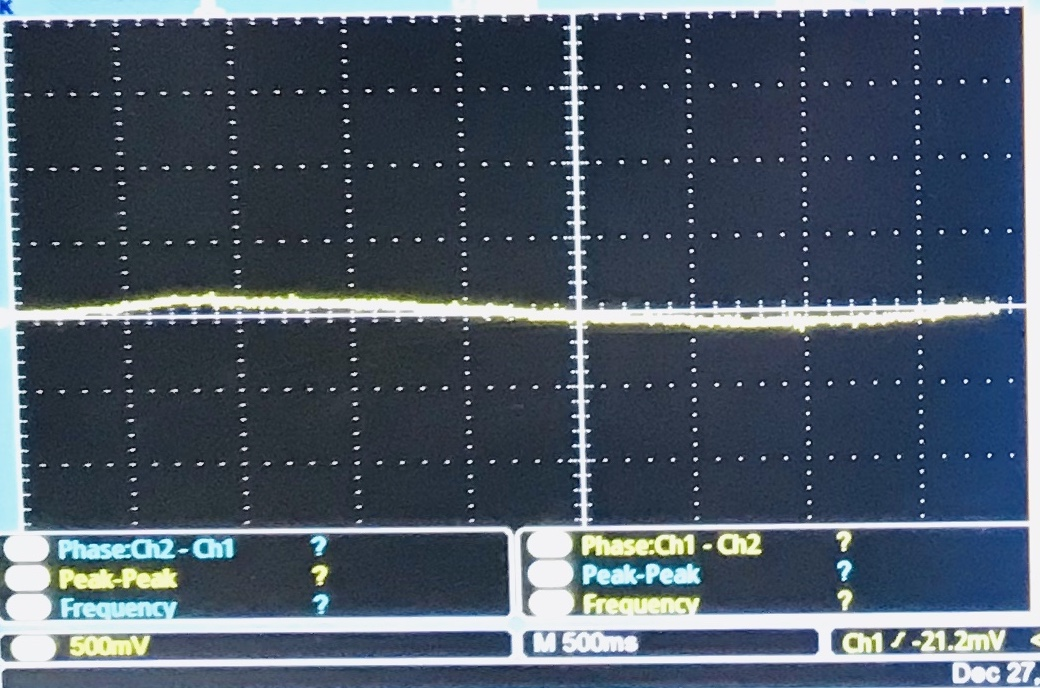
\includegraphics[width = 1.9in]{0-2.jpg}}&
\subfloat[0.3Hz]{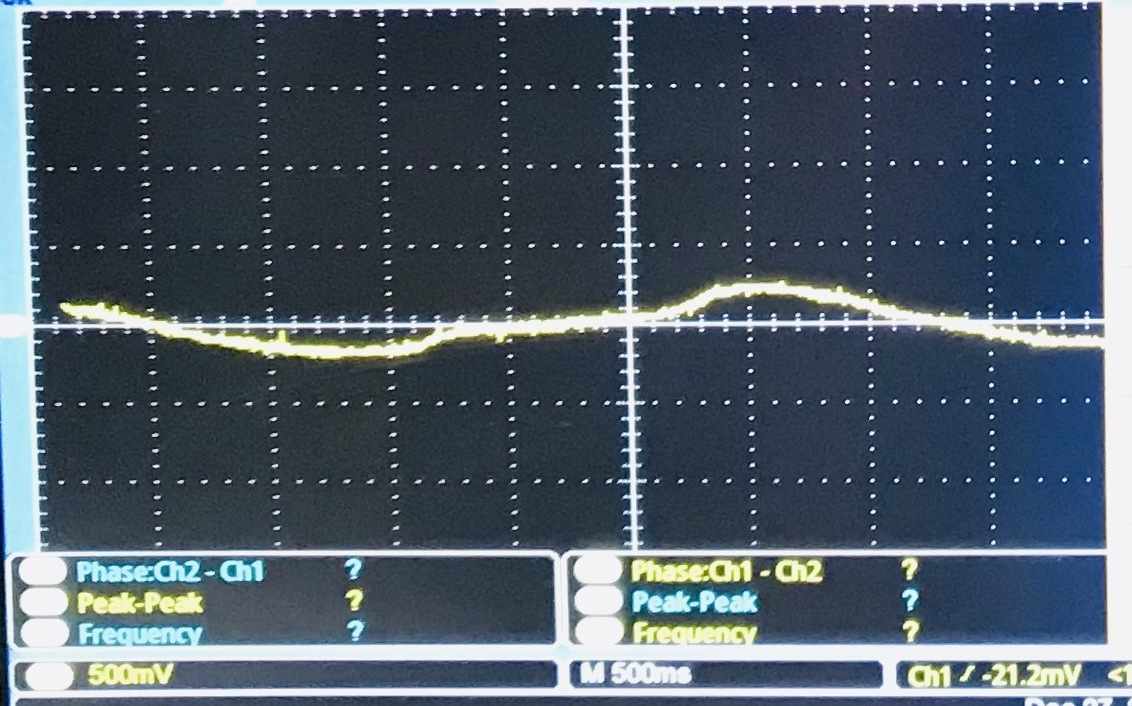
\includegraphics[width = 1.9in]{0-3.jpg}}\\

\end{tabular}
\end{figure}

\begin{figure}[h]
	\ContinuedFloat*
	\begin{tabular}{ccc}

\subfloat[0.4Hz]{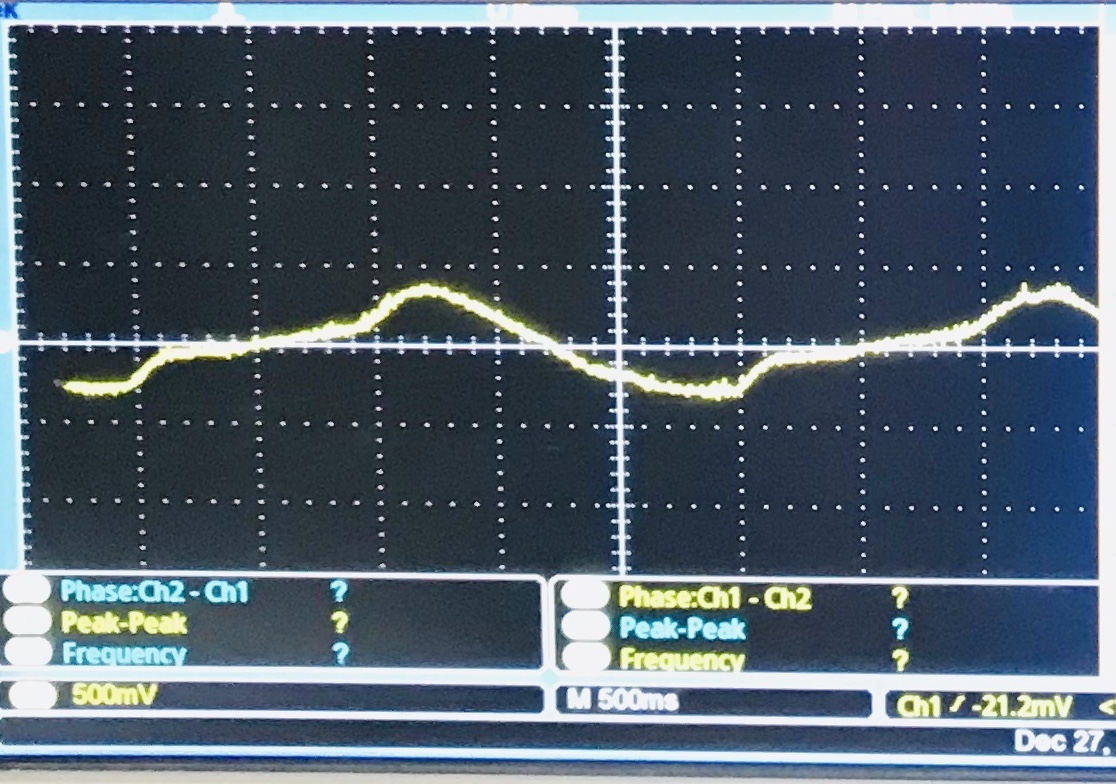
\includegraphics[width = 1.9in]{0-4.jpg}}&
\subfloat[0.5Hz]{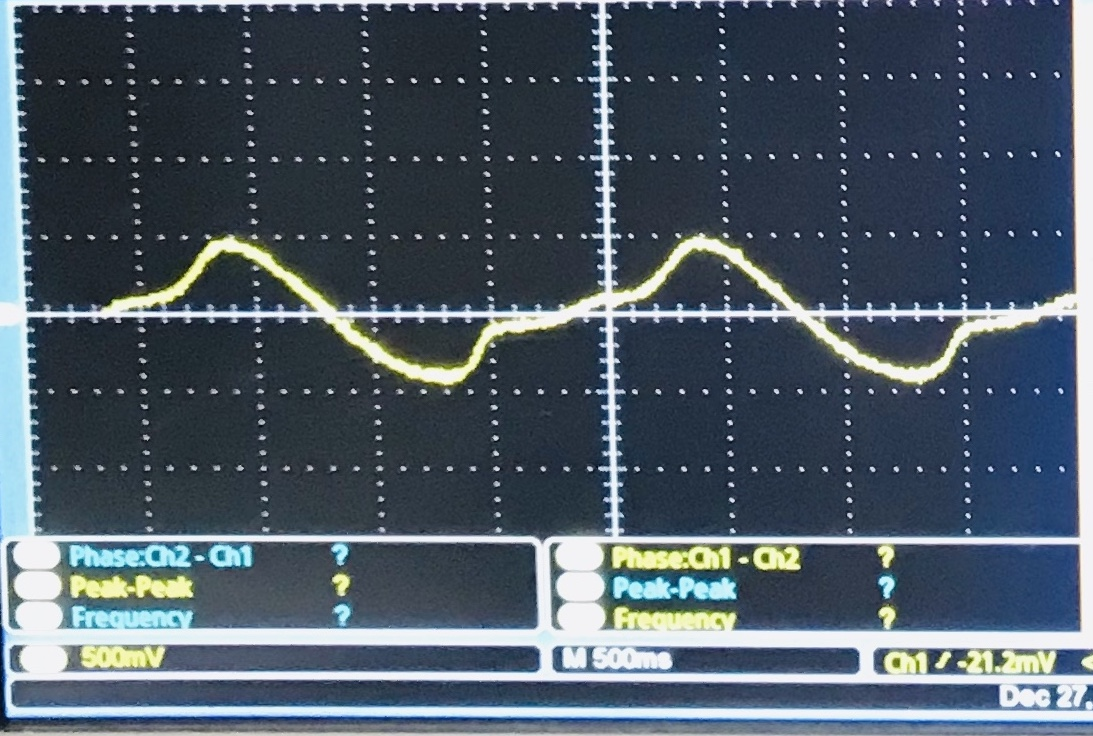
\includegraphics[width = 1.9in]{0-5.jpg}}&
\subfloat[0.6Hz]{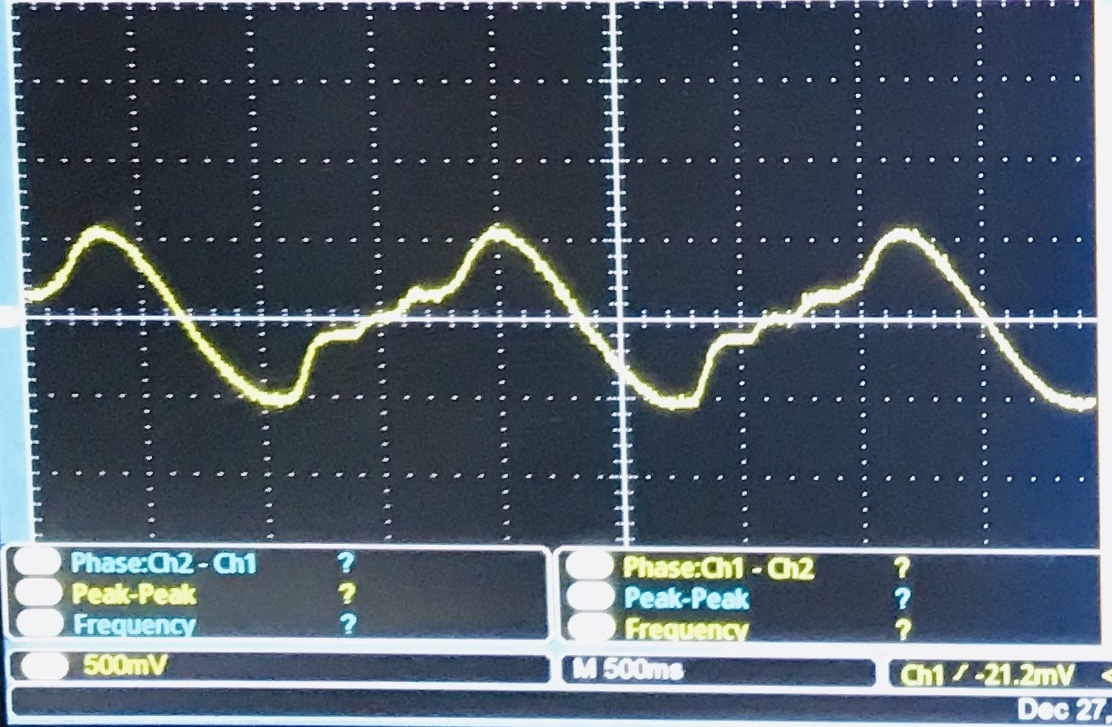
\includegraphics[width = 1.9in]{0-6.jpg}}\\

\subfloat[0.7Hz]{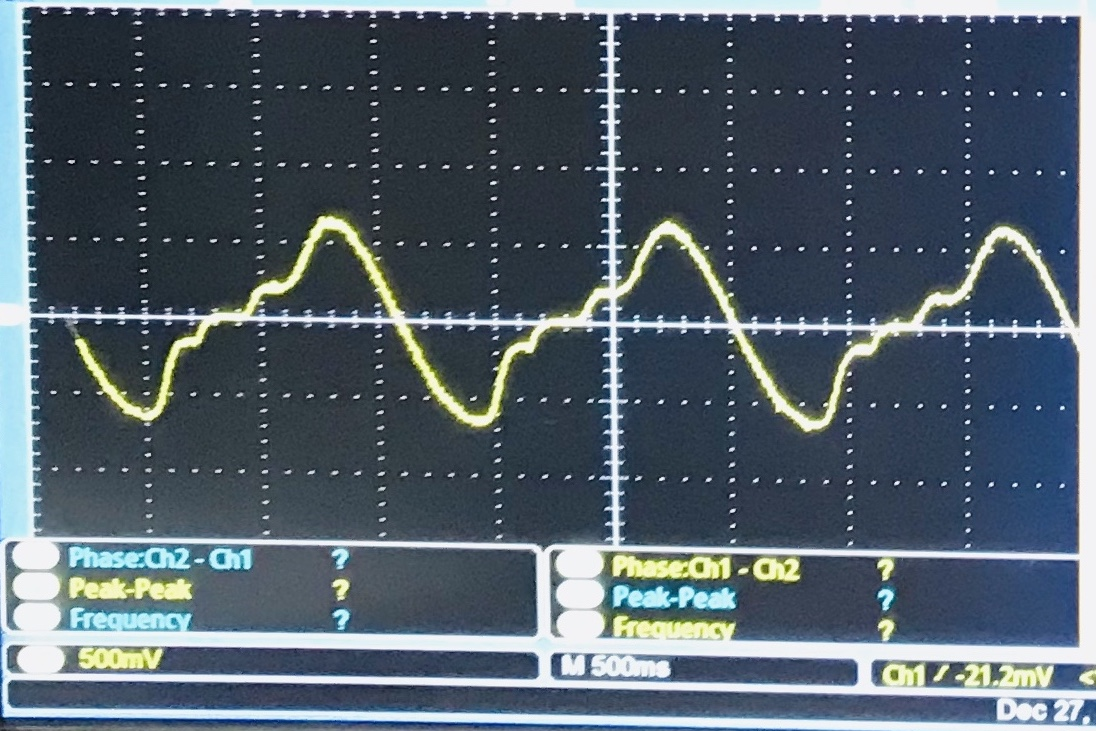
\includegraphics[width = 1.9in]{0-7.jpg}}&
\subfloat[0.9Hz]{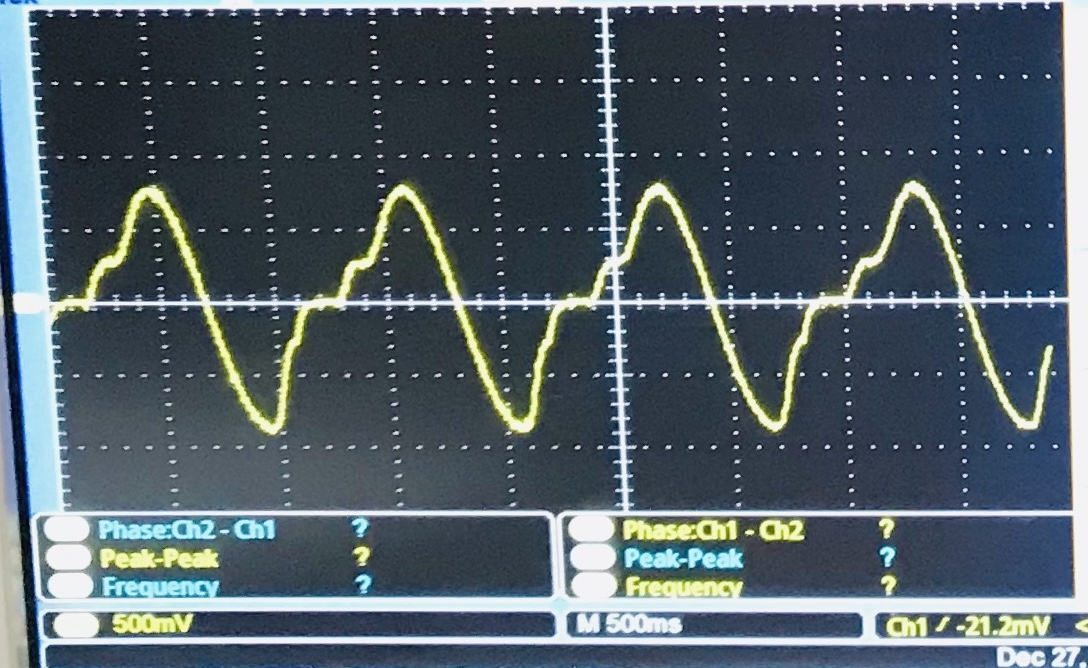
\includegraphics[width = 1.9in]{0-9.jpg}}&
\subfloat[1.2Hz ]{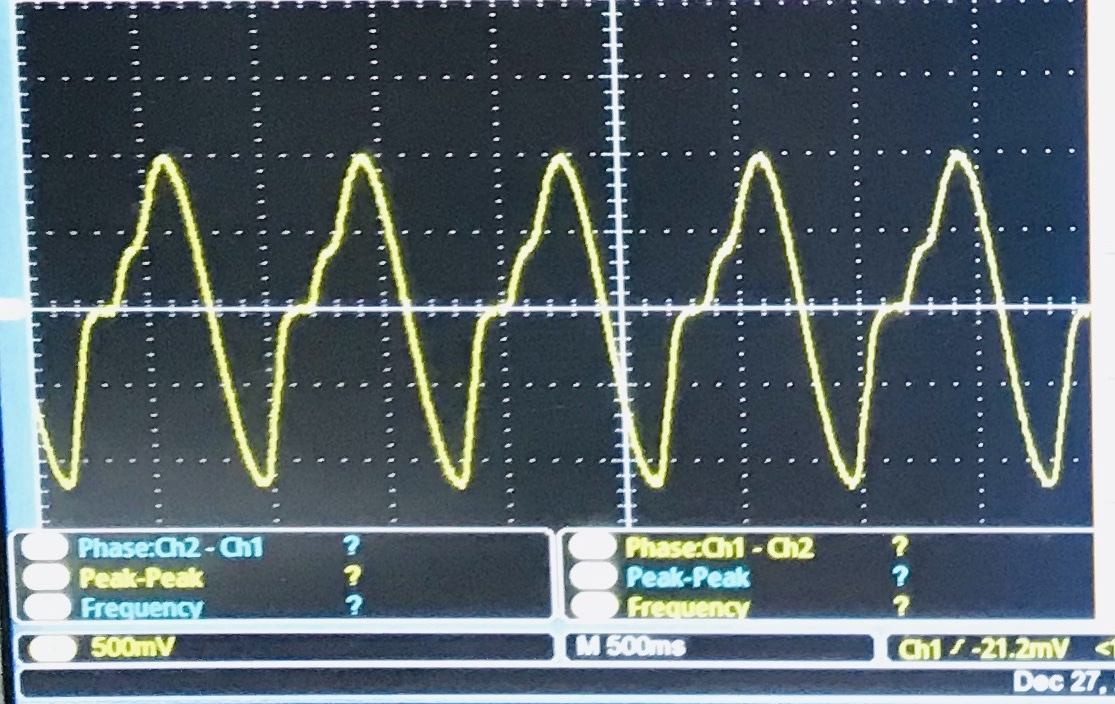
\includegraphics[width = 1.9in]{1-2.jpg}}\\

\subfloat[1.5Hz]{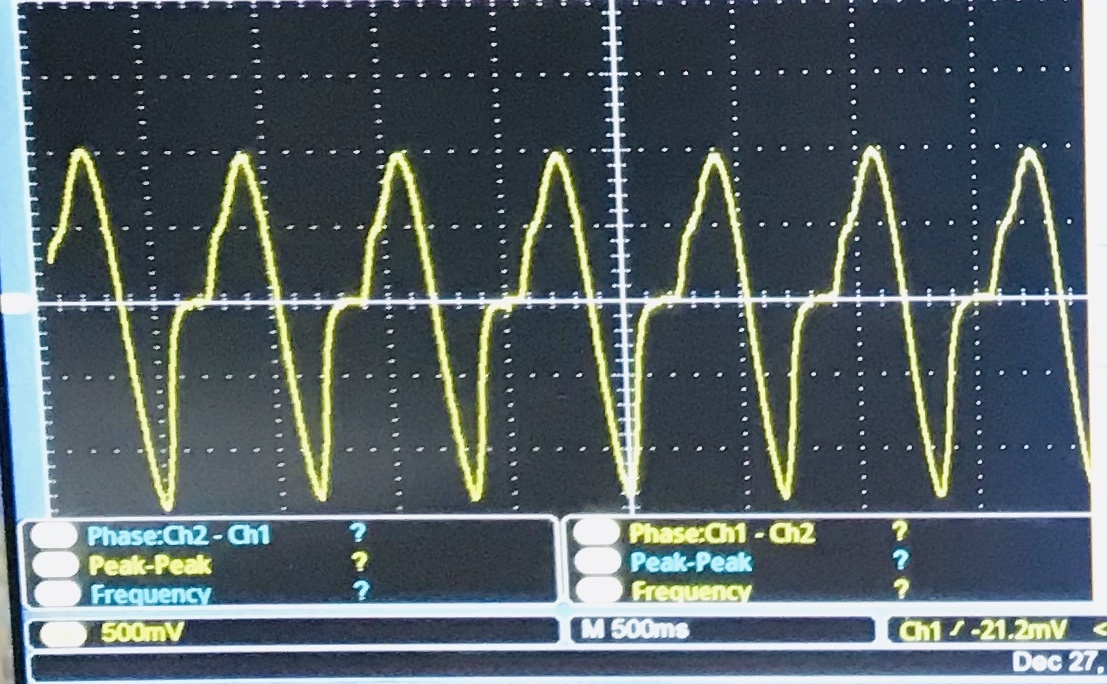
\includegraphics[width = 1.9in]{1-5.jpg}}&
\subfloat[2Hz]{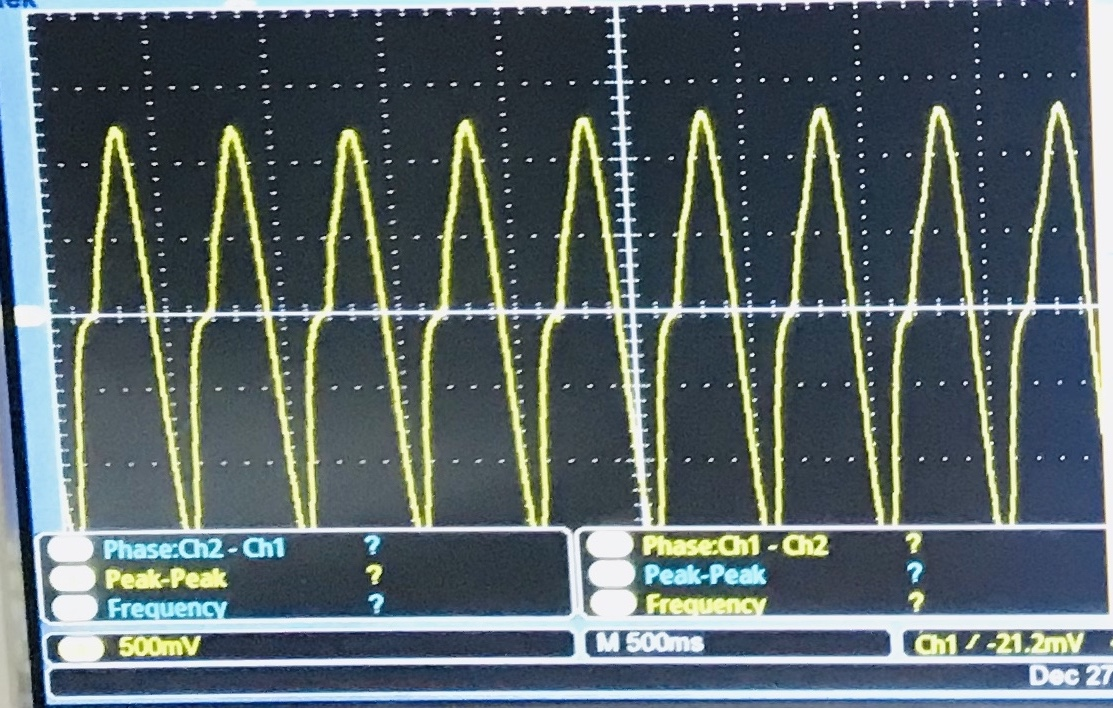
\includegraphics[width = 1.9in]{2.jpg}}&
\subfloat[2.5Hz]{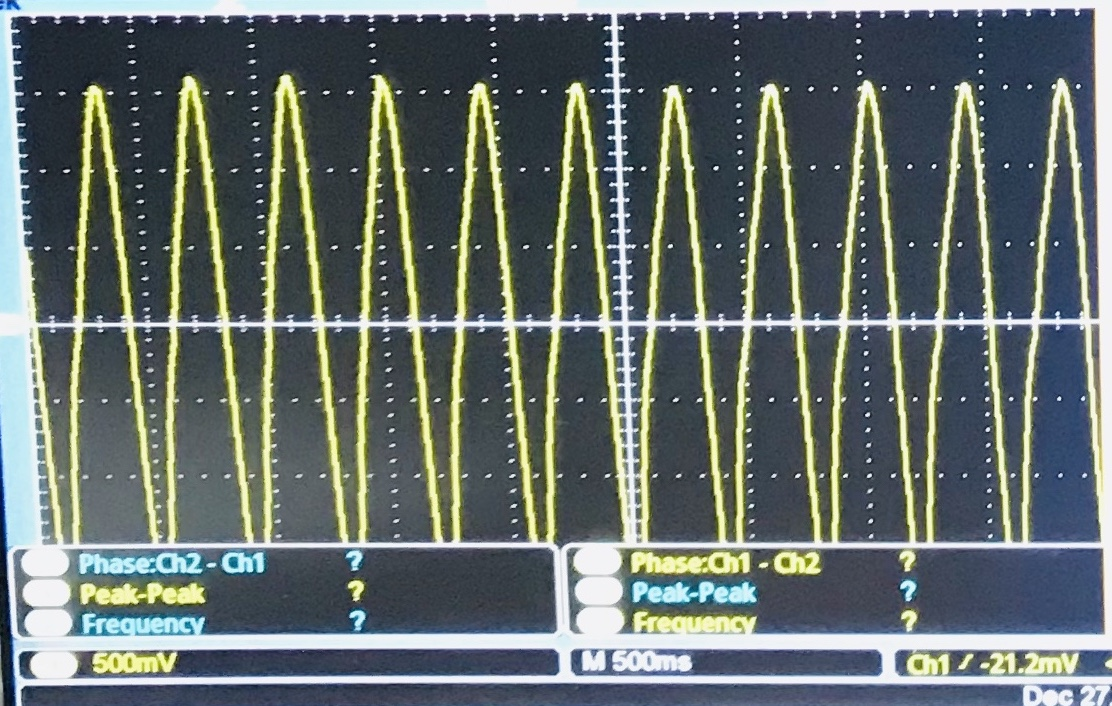
\includegraphics[width = 1.9in]{2-5.jpg}}\\

\subfloat[6Hz]{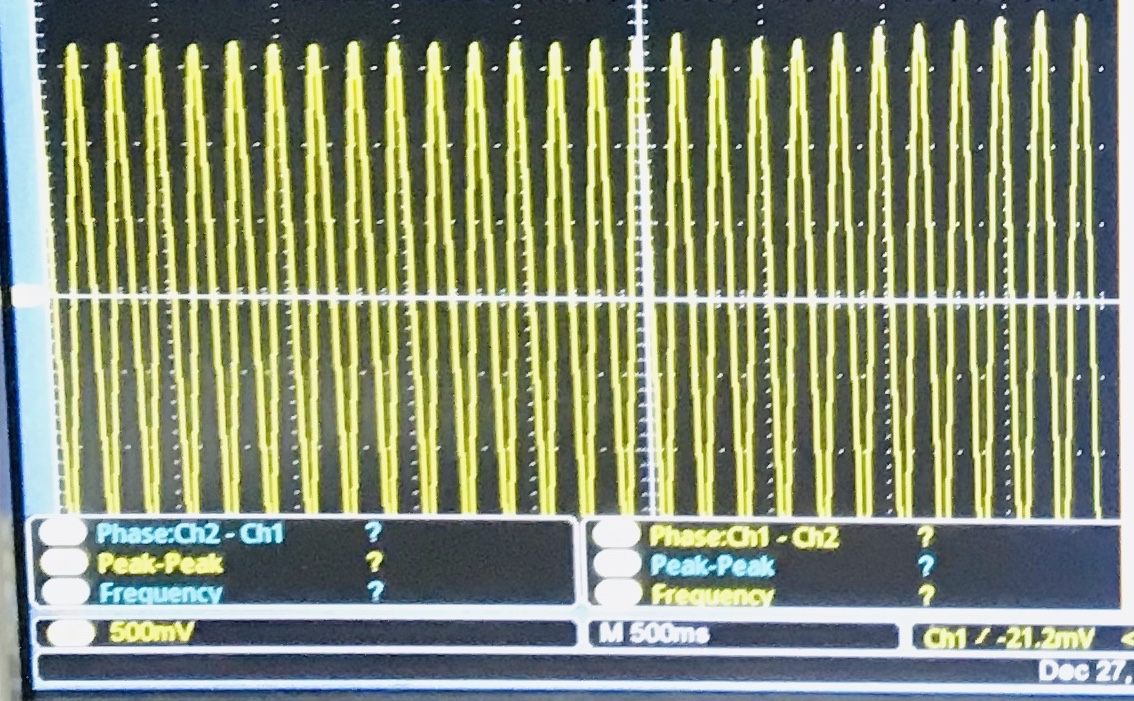
\includegraphics[width = 1.9in]{6.jpg}}&
\subfloat[10Hz]{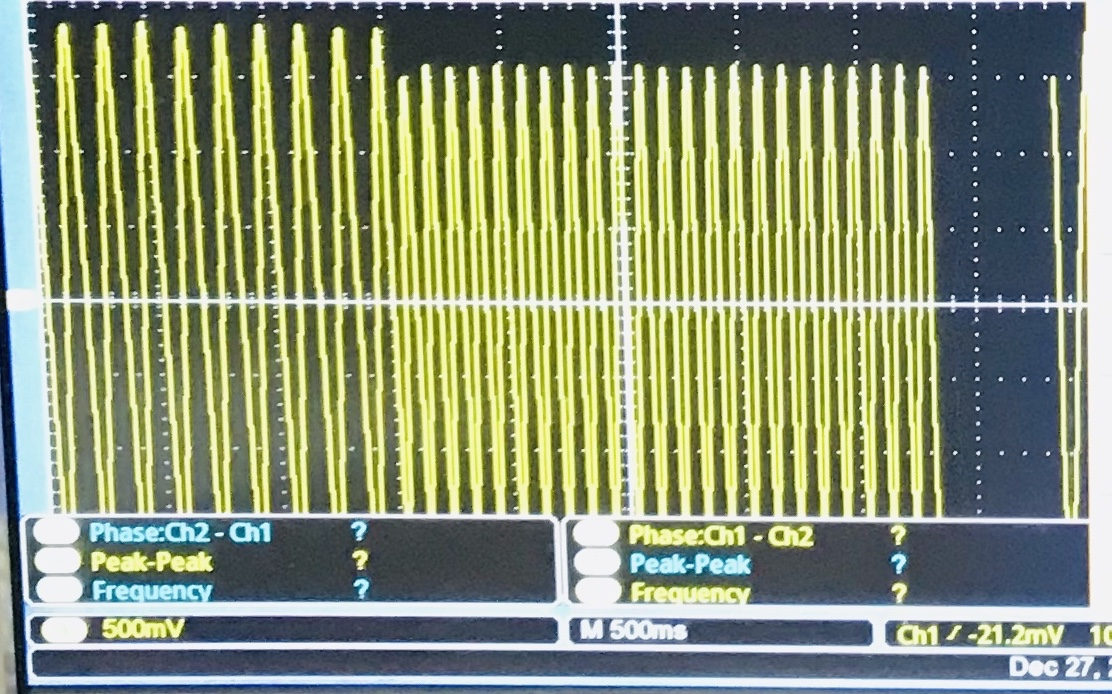
\includegraphics[width = 1.9in]{10.jpg}}&
\subfloat[15Hz]{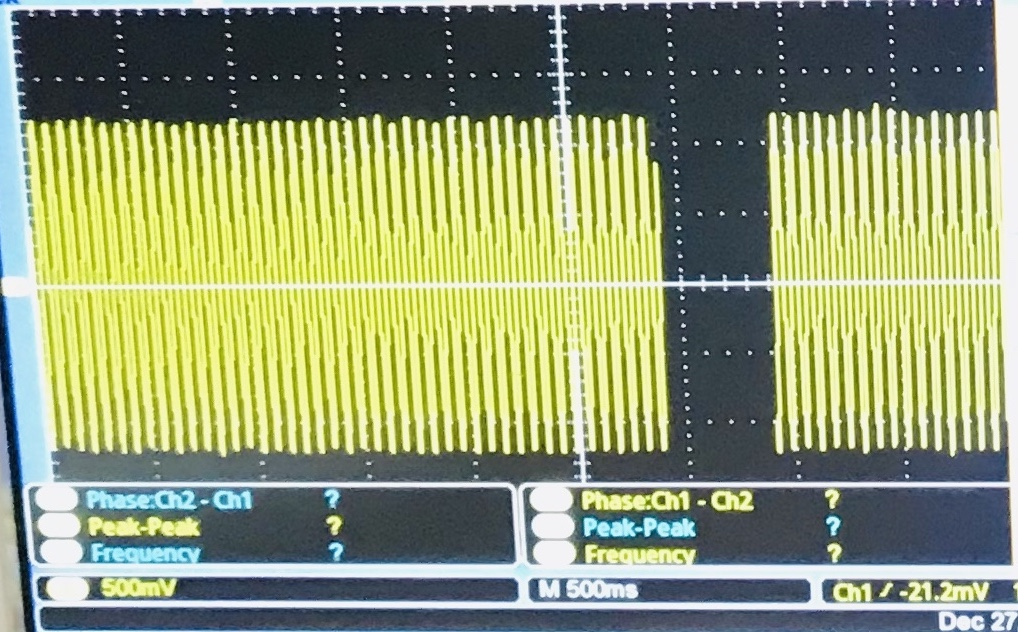
\includegraphics[width = 1.9in]{15.jpg}}\\

\end{tabular}
\caption{Frequency response of the bandpass filter}
	\end{figure}
\clearpage



By the observations above we were able to verify that the response of this circuit can be given by the graph below:

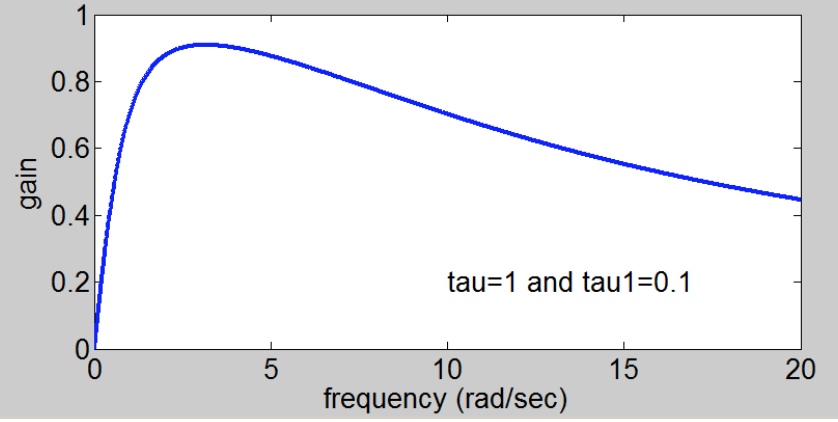
\includegraphics[scale=0.5]{bandpass.jpg}

\subsubsection{Obtaining a threshold value}

During testing, it was observed that due to ambient lighting conditions and movement of the patients’ finger placement between the LED and photodiode sudden amplitude changes can occur. 

It was evident that a hardcoded threshold value will not count the number of peaks accurately. Therefore, the calibration algorithm which was explained in \hyperref[sec:4.3.2]{4.3.2} determines a threshold value per session.


\begin{figure}[!htbp]
	
	\begin{tabular}{ccc}
\subfloat[Varying amplitudes]{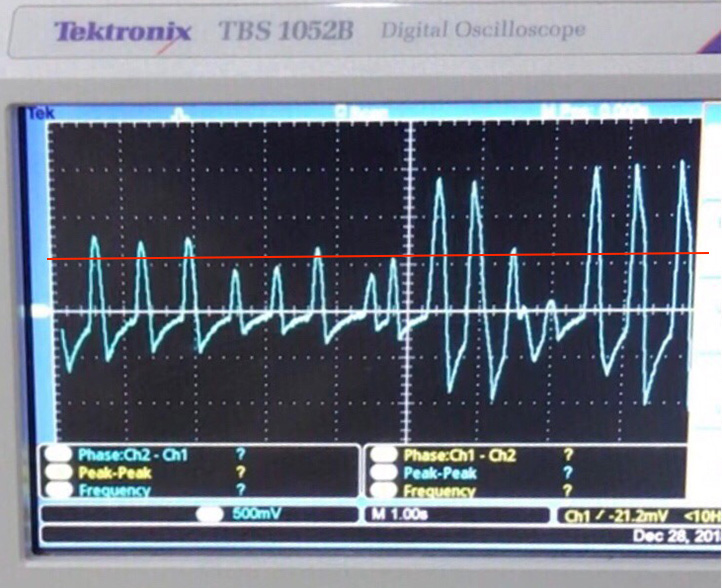
\includegraphics[width = 2.9in]{test1.jpg}}&
\subfloat[Amplitude Gradually decreasing]{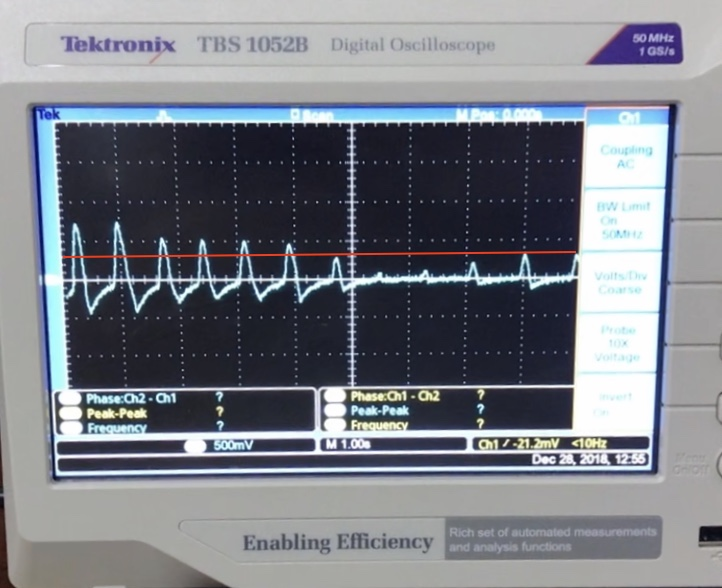
\includegraphics[width = 2.9in]{test2.jpg}}\\
	\end{tabular}
	\end{figure}
	
	

	\begin{wrapfigure}{L}{0.8\textwidth}
		\centering
		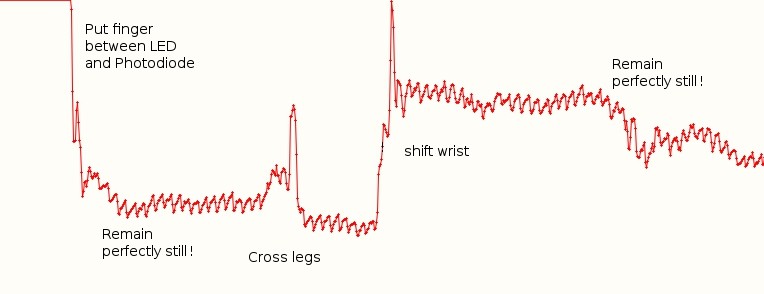
\includegraphics[width=0.75\textwidth]{breadboardmonitorwaveform.jpg}
		\caption{How PPG Varies\cite{analomy_pulse_sensor}}
		\end{wrapfigure}


		

\label{sec:results}
\begin{figure}[!htbp]
	\centering
	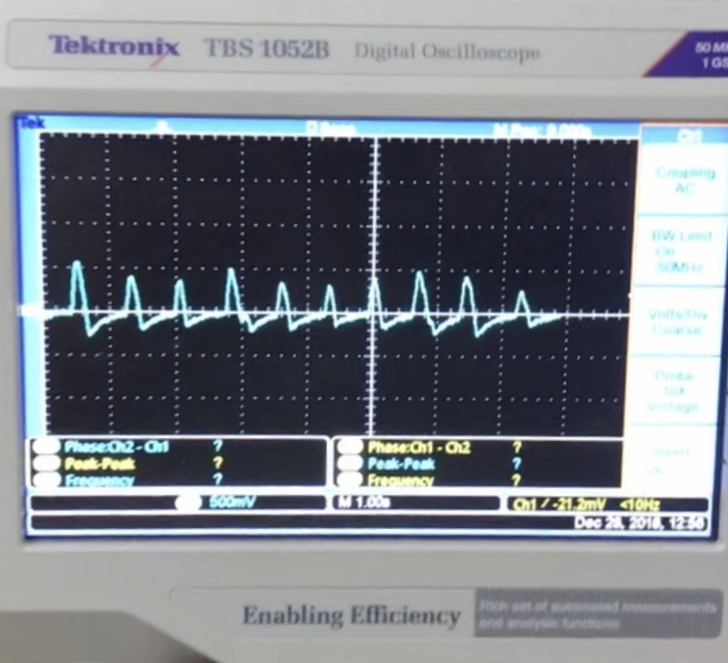
\includegraphics[scale = 0.35]{res1.jpg}
	\caption{Filtered Waveform}
\end{figure}

\clearpage


\newpage
\section{Discussion}
Using PPG we were able to monitor the heart rate with much accuracy and it seemed to be an easy method to be used for portable heart rate monitors. Since frequency of the analog waveform of the pulse that we receive of a person doesn’t exceed 2Hz the sampling frequency of 5Hz that we have used in this project seem to give the most accurate results. 
\\
Noise is the main issue that many faces when receiving analog signals and we were able to overcome that issue with the use of an appropriate active bandpass filter. The most difficult part of the project was to convert the analog signal a digital signal. Here we used a square regression line as the threshold and then counted the peaks.
\\
We used IR sensors to get the input signal from the fingertip, but it seems that using a green light PPG sensor will give a better input signal. Also, with the use of a smaller in size enclosure the heart rate monitor would be more convenient as a compatible device.
\\
As an improvement the use of a more advanced sensor would make this device output more accurate results.


\newpage
\section{Online Materials}
The project has been open sourced on Github. All the diagrams, schematics, PCB designs can be found through our repository.\\\\
\faGithub\href{https://github.com/ramithuh/Pulse-Sensor}{ https://github.com/ramithuh/Pulse-Sensor}.

 
\newpage
%	Bibliography


%----------------------------------------------------------------------------------------
\bibliography{biblist}{}
\bibliographystyle{plain}
\end{document}